\documentclass[a4paper]{article}
\usepackage[spanish,es-tabla]{babel}	% trabajar en español
\spanishsignitems	
%\usepackage{simplemargins}

%\usepackage[square]{natbib}
\usepackage{amsmath}
\usepackage{amsfonts}
\usepackage{amssymb}
\usepackage{bbold}
\usepackage{graphicx}
\usepackage{blindtext}
\usepackage{hyperref}

\begin{document}
\pagenumbering{gobble}

\Large
 \begin{center}
Reporte de Seminario 1\\
Computación Cuántica  

\hspace{10pt}

% Author names and affiliations
\large
Lic. Julio A. Medina$^1$ \\

\hspace{10pt}
\small  
$^1$ Universidad de San Carlos, Escuela de Ciencias Físicas y Matemáticas\\
Maestría en Física\\
\href{mailto:julioantonio.medina@gmail.com}{julioantonio.medina@gmail.com}\\

\end{center}

\hspace{10pt}

\normalsize
Durante el curso de Seminario 1 se han investigado los fundamentos teóricos de la computación cuántica. Se han repasado temas de mecánica estadística, como el concepto de ensambles, un tema recurrente en computación cuántica. La computación cuántica nace del deseo de Richcard P. Feynman de querer analizar y simular sistemas cuánticos por medio de sistemas informáticos, esto llevo rápidamente a la realización que el problema crecía exponencialmente con respecto al número de partículas a simular, esto implicaba que el costo computacional crecía de la misma manera, esto imposibilitó de gran manera simular dichos sistemas cuánticos. Feynman\cite{Feynman} publicó en 1981 un artículo seminal en el que plantó la semilla para crear sistemas de computación cuántica para simular mas efectivamente sistemas de naturaleza cuántica. \\

Se han revisado conceptos fundamentales y básicos de la computación cuántica como:
\begin{itemize}
\item El concepto del bit cuántico, \textbf{\textit{qubit}}.
\item Entrelazamiento cuántico.
\item Superposición de estados cuánticos.
\item Producto tensorial.
\item La esfera de Bloch.
\item Compuertas lógicas cuánticas.
\item Operador de Hadamard.
\item Teletransportación cuántica.
\item Transformada cuántica de Fourier.
\item Circuitos cuánticos.
\item Algoritmo de Shor.

\end{itemize} 
Ademas de la investigación teórica se han aprendido conceptos prácticos a través de la API para computación cuántica creada por IBM, Qiskit \cite{Qiskit}. Dicha API se usa como una biblioteca de python mediante la cual se pueden accesar a computadoras cuánticas reales en las instalaciones de IBM para poder probar y desarrollar circuitos cuánticos básicos. Este proyecto de seminario y tesis de maestría ha sido subido a un proyecto de GitHub donde también se han subido algunos scripts en python utilizando Qiskit donde se han desarrollado algoritmos como el de Deutch-Jozsa y otros, \url{https://github.com/Julio-Medina/Seminario}, esto con el fin de tener un historial claro del progreso de esta investigación.

\section{Inicios de la computación cuántica}
 La computación cuántica nace del deseo de Richcard P. Feynman de querer analizar y simular sistemas cuánticos por medio de sistemas informáticos, esto llevo rápidamente a la realización que el problema crecía exponencialmente con respecto al número de partículas a simular, esto implicaba que el costo computacional crecía de la misma manera, esto imposibilitó de gran manera simular dichos sistemas cuánticos. Feynman\cite{Feynman} publicó en 1981 un artículo seminal en el que plantó la semilla para crear sistemas de computación cuántica para simular mas efectivamente sistemas de naturaleza cuántica. \\
 
\section{De bits a Qubits}
En la computación clásica los estados o bits son $1$ o $0$, sin embargo en mecánica cuántica debido al principio de superposición de estados, se tiene que un qubit se puede encontrar en una superposición de estados i.e. simultáneamente estar en $1$ y $0$. Dichas superposiciones permiten realizar cálculos en varios estados simultáneamente, es decir se paralelizan los procesos de computo de una manera natural. Esto permite crear algoritmos cuánticos con mejoras exponenciales en el desempeño de computación. Sin embargo debido al colapso de la función de onda, cuando se hace una medición en los estados de superposición el estado colapsa en uno de los eigen-estados del operador que se utiliza para hacer la medición. \\
Debido a esto los algoritmos cuánticos se diseñan de tal manera que la respuesta correcta se amplifique, es decir que haya una resonancia de la respuesta correcta en la función de onda, esto hace que el diseño de algoritmos cuánticos sea una tarea poco trivial.
\subsection{Notación de Dirac}
Se utilizan para describir estados cuánticos. Son vectores en el espacio de Hilbert, pueden ser vectores con dimensiones finitas o describir cantidades continuas y ser vectores de dimensión infinita. El físico inglés Paul Dirac popularizó la llamada notación de Dirac para hacer los cálculos en mecánica cuántica mas compactos.
Se define al ket como
\begin{equation}
|a\rangle=
	\begin{pmatrix}
		a_1\\
		a_2
	\end{pmatrix}
\end{equation}
donde $a_1, a_2 \in \mathbb{C} $. Y el bra se define como el vector fila, o vector en el espacio dual del ket definido como 
\begin{equation}
\langle a|=
	\begin{pmatrix}
		a_1^*&a_2^*
	\end{pmatrix}
\end{equation}
donde $a_1^*, a_2^* \in \mathbb{C} $ son los complejos conjugados de $a_1, a_2$.
Los bra y los ket están relacionados de la siguiente manera
\begin{equation}
\langle a|=|a\rangle^\dagger
\end{equation}
que equivale a 
\begin{equation}
\begin{pmatrix}
		a_1\\
		a_2
	\end{pmatrix}^\dagger=
	\begin{pmatrix}
		a_1^*&a_2^*
	\end{pmatrix}
\end{equation}
donde $a_1=x+iy$ y $a_1^*=x-iy$ es el complejo conjugado, el operador $\dagger$ da el transpuesto conjugado de un vector o matriz.\\
%\subsubsection{BraKet}
Se define al braket como el producto interno o producto escalar en el espacio de Hilbert.
\begin{equation}
\langle b | a\rangle=a_1b_1^*+a_2b_2^*=\langle a | b\rangle^*\in \mathbb{C}
\end{equation}.
El ketbra o producto abierto se define como 
\begin{equation}
|a\rangle\langle b|=
	\begin{pmatrix}
		a_1 b_1^*& a_1 b_2^*\\
		a_2 b_1^*& a_2 b_2^*\\
	\end{pmatrix}
\end{equation}
\subsection{Representación de Qubit}
La representación de un qubit viene dada naturalmente por los spinores utilizados para describir el experimento de Stern-Gerlach en el que se miden el spin de átomos de plata. Estos spinores se definen como 
\begin{equation}\label{eq::qubit0}
|0\rangle\equiv
\begin{pmatrix}
		1\\
		0
	\end{pmatrix}
\end{equation}
como el análogo cuántico del estado $0$ para un bit clásico, y para el estado clásico $1$ se usa
\begin{equation}\label{eq::qubit1}
|1\rangle\equiv
\begin{pmatrix}
		0\\
		1
	\end{pmatrix}
\end{equation}
estos estados cuánticos son evidentemente ortonormales $\langle 0 | 1\rangle=0$ y $\langle 0 | 0\rangle=\langle 1 | 1\rangle=1$. Se nota que estos dos estados forman una base. Todos los estados cuánticos están normalizados
\begin{equation}
\langle \psi | \psi\rangle=1
\end{equation}
por ejemplo $|\psi\rangle=\frac{1}{\sqrt{2}}(|0\rangle+|1\rangle)$.
\section{Mediciones}
Por lo general se utilizan bases ortonormales para describir y medir estados cuánticos, aquí se sigue esa convención. Durante una medición en la base $\{|0\rangle, |1\rangle\}$ el estado colapsara ya sea a $|0\rangle$ o $|1\rangle$, estos son los eigen-estados de $\sigma_z$ la matriz Pauli-z(ver \ref{sec::PauliMatrix}) a esto se le conoce como medición en z.\\
Hay infinitas bases distintas en las que se pueden realizar las mediciones pero otras bases comunes son $\{|+\rangle, |-\rangle \}$ definidas como:
\begin{equation}
|+\rangle\equiv\frac{1}{\sqrt{2}}(|0\rangle+|1\rangle)
\end{equation}
\begin{equation}
|-\rangle\equiv\frac{1}{\sqrt{2}}(|0\rangle-|1\rangle)
\end{equation}
que son los eigen-vectores de la matriz de Pauli x $\sigma_x$, y como se ha de esperar otra base comúnmente usada son los eigen-vectores de la matriz Pauli $y$, $\sigma_y$:
\begin{equation}
|+i\rangle\equiv\frac{1}{\sqrt{2}}(|0\rangle+i|1\rangle)
\end{equation}
\begin{equation}
|-i\rangle\equiv\frac{1}{\sqrt{2}}(|0\rangle-i|1\rangle)
\end{equation}
\subsection{Regla de Born}
La probabilidad que el estado $|\psi\rangle$ colapse durante una medición proyectiva en la base $\{|x\rangle, |x^+ \rangle \}$ al estado $|x\rangle$ está dada por
\begin{equation}
P(x)=|\langle x|\psi\rangle|^2
\end{equation}
y del hecho que se está trabajando con estados normalizados se tiene, como es de esperarse que
\begin{equation}
\sum_i P(x_i)=1
\end{equation}
Para ilustrar esto se presentan algunos ejemplos:\\
a. El estado $|\psi\rangle=\frac{1}{\sqrt{3}}(|0\rangle +\sqrt{2}|1\rangle)$ es medido en la base $\{|0\rangle,   |1\rangle \}$ calcule las probabilidades correspondientes:
\begin{equation*}
P(0)=\bigg |\langle 0|\frac{1}{\sqrt{3}}(|0\rangle +\sqrt{2}|1\rangle)\bigg |^2=\bigg|\frac{1}{\sqrt{3}}\langle 0|0\rangle+\sqrt{\frac{2}{3}}\langle 0|1\rangle \bigg |^2
\end{equation*}
\begin{equation*}
P(0)=\bigg|\frac{1}{\sqrt{3}} \bigg|^2=\frac{1}{3}
\end{equation*}
\begin{equation*}
P(1)=\bigg|\sqrt{\frac{2}{3}} \bigg|^2=\frac{2}{3}
\end{equation*}
\begin{equation*}
P(0)+P(1)=1
\end{equation*}
b. El estado $|\psi\rangle=\frac{1}{\sqrt{2}}(|0\rangle-|1\rangle)$ es medido en la base $\{|+\rangle, |-\rangle\}$, encontrar las probabilidades correspondientes:
\begin{equation*}
P(+)=\bigg| \langle +|\psi\rangle\bigg|^2=\bigg|\frac{1}{\sqrt{2}}(\langle 0| +\langle 1|)\cdot \frac{1}{\sqrt{2}}(|0\rangle -|1\rangle|)\bigg|^2
\end{equation*}
\begin{equation*}
P(+)=\frac{1}{4}\bigg|\langle 0|0\rangle-\langle 0|1\rangle+\langle 1|0\rangle-\langle 1|1\rangle\bigg|^2=0
\end{equation*}
\begin{equation*}
P(-)=1
\end{equation*}
Como es de esperarse ya que $\bigg| \langle -|\psi\rangle\bigg|^2=\bigg| \langle -|-\rangle\bigg|^2=1$ y $\bigg| \langle +|-\rangle\bigg|^2=0$ por la propiedad de ortogonalidad de estas bases.

\section{Circuitos Cuánticos}
Se utiliza el "modelo de circuitos", una secuencia de bloques básicos que realizan los cómputos elementales, a estos bloques básicos se les conoce como compuertas.
\subsection{Compuertas de un solo Qubit}
Para hacer una analogía con las compuertas lógicas clásicas se presenta la compuerta lógica NOT, representada por \ref{fig::NOT_gate}, 
\begin{figure}[h]
\begin{center}
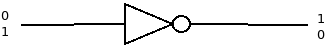
\includegraphics[scale=0.4]{./classicalNOT.png} 
\end{center} 
\caption{Compuerta NOT}
\label{fig::NOT_gate}
\end{figure}
como se puede ver en la figura la operación que realiza el operador NOT en un bit es trivial, invierte el estado de bit de 0 a 1 y viceversa.
Una de las características fundamentales de la teoría cuántica es el hecho que es unitaria, es decir que los operadores cuánticos, en este caso las compuertas cuánticas tienen que ser operadores unitarios(matrices unitarias), es decir que para un operador $U$ se cumple que:
\begin{equation}
U^\dagger U=\mathbb{1}
\end{equation}
esto implica que cuando un operador unitario actúa sobre un ket, no se cambia la magnitud del ket. De la notación de Dirac se puede representar a un operador unitario $U$ como  una combinación lineal de ketbras de la siguiente manera
\begin{equation}
U=
	\begin{pmatrix}
		u_{00} &u_{01} \\
		u_{10} &u_{11}
	\end{pmatrix}=u_{00}|0\rangle\langle 0|+u_{01}|0\rangle\langle 1|+u_{10}|1\rangle\langle 0|+
	u_{11}|1\rangle\langle 1|
\end{equation}
\subsubsection{Matrices de Pauli}\label{sec::PauliMatrix}
La matriz de Pauli x, $\sigma_x$ esta definida como 
\begin{equation}
\sigma_x=\begin{pmatrix}
		0 &1 \\
		1 &0
	\end{pmatrix}=|0\rangle\langle 1|+|1\rangle\langle 0|
\end{equation}
esta matriz sirve como el análogo cuántico de la compuerta NOT, para ver esto basta con operar con la representación de los qubits definida en \ref{eq::qubit0} y \ref{eq::qubit1}:
\begin{equation}
\sigma_x|0\rangle=
	\begin{pmatrix}
		0 &1 \\
		1 &0
	\end{pmatrix}
	\begin{pmatrix}
		1 \\
		0
	\end{pmatrix}=
	\begin{pmatrix}
		0 \\
		1
	\end{pmatrix}=|1\rangle
\end{equation}
De igual manera usando la notación de Dirac se tiene que
\begin{equation}
\sigma_x|1\rangle=(|0\rangle\langle 1|+|1\rangle\langle 0|)|1\rangle=|0\rangle
\end{equation}
este comportamiento también se conoce como un bit-flip(intercambio de bit), también se puede actuar en superposiciones, los eigen-vectores de $\sigma_x$ son los kets $|+\rangle, |-\rangle$.\\
La matriz de Pauli z, $\sigma_z$ está definida como 
\begin{equation}
\sigma_z=
	\begin{pmatrix}
		1 &0 \\
		0 &-1
	\end{pmatrix}=|0\rangle\langle 0|-|1\rangle\langle 1|
\end{equation}
el comportamiento de esta matriz se describe como un intercambio de fase(phase-flip), para visualizar esto actúa sobre la base $\{|+\rangle, |-\rangle\}$:
\begin{equation}
\sigma_z|+\rangle=
	\begin{pmatrix}
		1 &0 \\
		0 &-1
	\end{pmatrix}\frac{1}{\sqrt{2}}
	\begin{pmatrix}
		1 \\
		1
	\end{pmatrix}=\frac{1}{\sqrt{2}}
	\begin{pmatrix}
		1 \\
		-1
	\end{pmatrix}=|-\rangle
\end{equation}
en notación de Dirac se tiene
\begin{equation}
\sigma_z|-\rangle=(|0\rangle\langle 0|-|1\rangle\langle 1|)\frac{1}{\sqrt{2}}(|0\rangle-|1\rangle)=\frac{1}{\sqrt{2}}(|0\rangle+|1\rangle)=|+\rangle
\end{equation}
Los eigen-vectores de la matriz $\sigma_z$ son los kets $|0\rangle, |1\rangle$.\\
La matriz Pauli y, $\sigma_y$ está definida por
\begin{equation}
\sigma_y=
	\begin{pmatrix}
		0 &-i \\
		i & 0
	\end{pmatrix}=i|1\rangle\langle 0|-i|0\rangle\langle 1|
\end{equation}
Se hace la observación que $\sigma_y=i \sigma_x\sigma_z$ por lo que se puede interpretar a esta compuerta como una sucesión de bit flip y phase flip. \\
Cualquiera de las matrices de Pauli $\sigma_x, \sigma_y, \sigma_z$ cumple con 
\begin{equation}
\sigma_i^2=\mathbb{1}
\end{equation}
El conjunto de las matrices de Pauli y la matriz identidad forman una base de matrices de $2\times2$.
\subsubsection{Compuerta de Hadamard}
La compuerta de Hadamard, $H$ está definida por
\begin{equation}
	H=
	\frac{1}{\sqrt{2}}
	\begin{pmatrix}
		1 & 1 \\
		1 &-1
	\end{pmatrix}=\frac{1}{\sqrt{2}}(|0\rangle\langle 0|+|0\rangle\langle 1|+|1\rangle\langle 0|-|1\rangle\langle 1|)
\end{equation}
la compuerta de Hadamard es muy útil ya que crea superposiciones de qubits, esto se ejemplifica de la siguiente manera
\begin{equation}
H|0\rangle=\frac{1}{\sqrt{2}}(|0\rangle\langle 0|+|0\rangle\langle 1|+|1\rangle\langle 0|-|1\rangle\langle 1|)|0\rangle=\frac{1}{\sqrt{2}}(|0\rangle+|1\rangle)
\end{equation}
\begin{equation}
H|0\rangle=|+\rangle
\end{equation}
de igual manera se tiene que 
\begin{equation}
H|1\rangle=|-\rangle
\end{equation}
Debido que a que toda compuerta cuántica es unitaria y añadido al hecho que $H$ es un operador Hermitico, i.e. $H^\dagger=H$, se tiene que 
\begin{equation}
H|+\rangle=|0\rangle
\end{equation}
\begin{equation}
H|-\rangle=|1\rangle
\end{equation}
de esto que la compuerta de Hadamard pueda ser utilizada para cambiar entre las bases $x$ y $z$.
\subsection{Estados cuánticos de multipartículas}
Para describir estados cuánticos de multipartículas se utiliza el producto tensorial, es decir que si tengo un estado para una partícula $|a\rangle$ y otro estado para una partícula distinta $|b\rangle$ se tiene que el estado bipartito se da por
\begin{equation}
|a\rangle \otimes |b\rangle=
	\begin{pmatrix}
		a_1 \\
		a_2
	\end{pmatrix}\otimes
	\begin{pmatrix}
		b_1 \\
		b_2
	\end{pmatrix}=
	\begin{pmatrix}
		a_1 b_1 \\
		a_1 b_2 \\
		a_2 b_1 \\
		a_2 b_2 
	\end{pmatrix}
\end{equation}
Para ejemplificar esto, supongamos que se tiene al sistema A en el estado $|1\rangle_A$ y al sistema B en el estado $|0\rangle_B$, entonces el estado total(híbrido) del sistema está dado por
\begin{equation}
|10\rangle_{AB}\equiv |1\rangle_A\otimes |0\rangle_B=
	\begin{pmatrix}
		0 \\
		0\\
		1\\
		0
	\end{pmatrix}	
\end{equation}
como una observación importante de estos estados es que se les llama no correlacionados, también hay estados bipartitos que no pueden escribirse como $|\psi\rangle_A\otimes|\psi\rangle_B$, estos se conocen como estados correlacionados y para estados puros son estados entrelazados.\\
\subsection{Compuertas de dos Qubits}
Para hacer una analogía con compuertas lógicas clásicas se presenta a la compuerta lógica XOR, con una tabla de verdad dada por 
\begin{center}
\begin{tabular}{ |c|c|c| } 
 \hline
 $x$ & $y$ & $x\oplus y$ \\ \hline
 0   & 1   &   1\\
 1   & 0   &   1\\
 0   & 0   &   0\\
 1   & 1   &   0\\ 
 \hline
\end{tabular}
\end{center}
se nota que el operador XOR es un operador no reversible, sin embargo como ya se discutió anteriormente le teoría cuántica es unitaria y por lo tanto reversible. Para resolver este inconveniente se tiene la siguiente compuerta cuántica de dos qubits, llamada CNOT(controlled NOT), definida por
\begin{equation}
\text{CNOT}=
	\begin{pmatrix}
		1 & 0 & 0 & 0 \\
		0 & 1 & 0 & 0 \\
		0 & 0 & 0 & 1 \\
		0 & 0 & 1 & 0
	\end{pmatrix}=|00\rangle\langle 00|+|01\rangle\langle 01|+|10\rangle\langle 11|+|11\rangle\langle 10|
\end{equation}
para ver el efecto que la compuerta cuántica CNOT tiene se realizan los siguientes cálculos detalladamente:
\begin{equation}
\text{CNOT}|00\rangle_{xy}=(|00\rangle\langle 00|+|01\rangle\langle 01|+|10\rangle\langle 11|+|11\rangle\langle 10|)|00\rangle
\end{equation}
\begin{equation*}
\text{CNOT}|00\rangle=|00\rangle_{xy}
\end{equation*}
de igual manera se tiene que 
\begin{equation}
\text{CNOT}|10\rangle_{xy}=(|00\rangle\langle 00|+|01\rangle\langle 01|+|10\rangle\langle 11|+|11\rangle\langle 10|)|10\rangle_{xy}
\end{equation}
\begin{equation*}
\text{CNOT}|10\rangle=|11\rangle_{xy}
\end{equation*}
\begin{equation}
\text{CNOT}|01\rangle_{xy}=(|00\rangle\langle 00|+|01\rangle\langle 01|+|10\rangle\langle 11|+|11\rangle\langle 10|)|01\rangle_{xy}
\end{equation}
\begin{equation*}
\text{CNOT}|01\rangle=|01\rangle_{xy}
\end{equation*}
\begin{equation}
\text{CNOT}|11\rangle_{xy}=(|00\rangle\langle 00|+|01\rangle\langle 01|+|10\rangle\langle 11|+|11\rangle\langle 10|)|11\rangle_{xy}
\end{equation}
\begin{equation*}
\text{CNOT}|11\rangle=|10\rangle_{xy}
\end{equation*}

Estos resultados se pueden resumir en la siguiente tabla, donde las dos primeras columnas representa la entrada y las últimas representan la salida de la operación, en este caso con el qubit de control, es decir el qubit del sistema x, se tiene un análogo de la compuerta XOR que en este caso es reversible como se puede ver en la tabla de verdad.
\begin{center}
\begin{tabular}{ |c|c|c|c| } 
 \hline
 $x$ & $y$ & $x$ & $x\oplus y$ \\ \hline
 0   & 1   &  0 &    1\\
 1   & 0   &  1 &    1\\
 0   & 0   &  0 &    0\\
 1   & 1   &  1 &    0\\ 
 \hline
\end{tabular}
\end{center}
Una representación gráfica de la compuerta CNOT realizada con la API de computación cuántica Qiskit se puede ver en la siguiente figura:
\begin{figure}[h]
\begin{center}
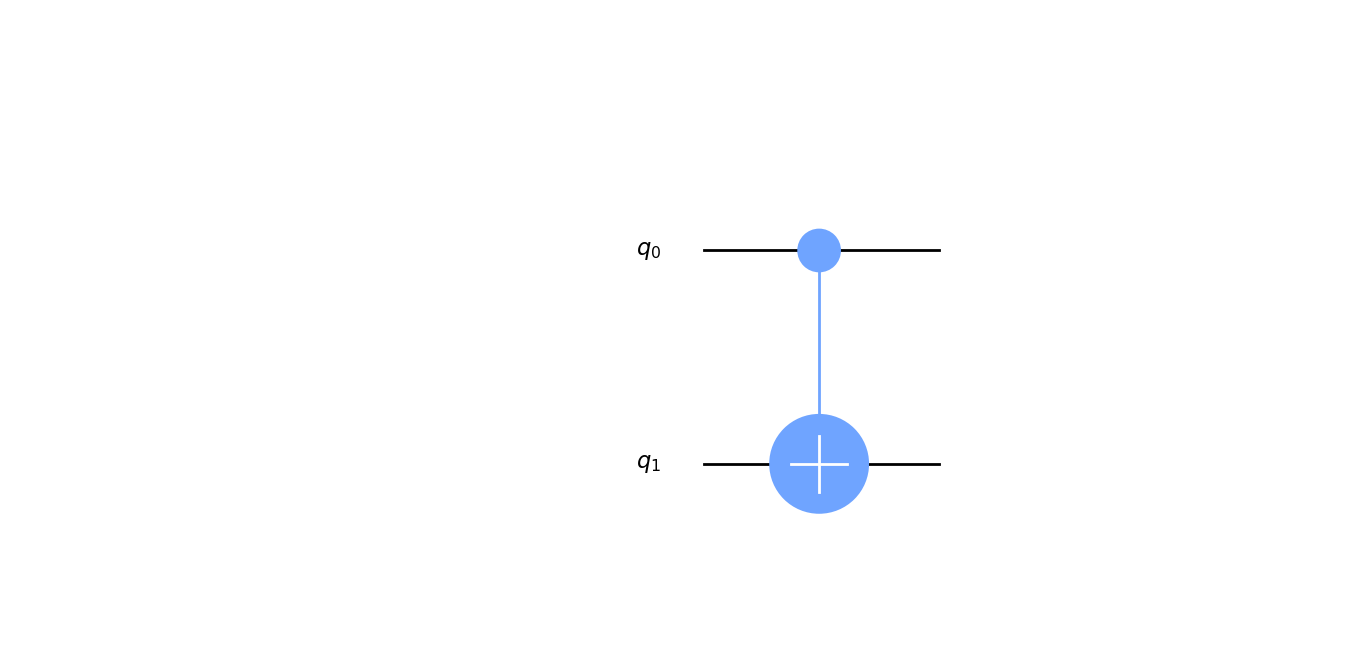
\includegraphics[scale=0.29]{./basic_CNOT_circuit.png} 
\end{center} 
\caption{Compuerta cuántica CNOT}
\label{fig::NOT_gate}
\end{figure}\\
Es posible demostrar que los circuitos cuánticos pueden calcular cualquier función clásica de álgebra boolena, el fundamento de los circuitos digitales y por ende de toda computadora clásica.

\section{Entrelazamiento cuántico}
Si un estado  puro $|\psi\rangle_{AB}$ de los sistemas A y B no puede escribirse como $|\phi\rangle_A\otimes |\gamma\rangle_B$ entonces el estado $|\psi\rangle_{AB}$ se conoce como un estado entrelazado, que es la definición para un estado correlacionado, pero ya que se está tratando solo con estado puros todo estado correlacionado es también un estado entrelazado.
\subsection{Estados de Bell}
Hay cuatro estados llamados Estados de Bell, en honor al físico John Bell. Bell desarrollo las también llamadas desigualdades de Bell \cite{Bell}, con las que resolvió la paradoja de Einstein-Podolsky-Rosen. Los llamados estados de Bell están máximamente entrelazados, es decir que violan las desigualdades de Bell exactamente, aparte estos estados de Bell forman una base ortonormal. Se definen como
\begin{equation}\label{eq::bell1}
|\psi^{00}\rangle\equiv \frac{1}{\sqrt{2}}(|00\rangle+|11\rangle)
\end{equation}
\begin{equation}\label{eq::bell2}
|\psi^{01}\rangle\equiv \frac{1}{\sqrt{2}}(|01\rangle+|10\rangle)
\end{equation}
\begin{equation}\label{eq::bell3}
|\psi^{10}\rangle\equiv \frac{1}{\sqrt{2}}(|00\rangle-|11\rangle)
\end{equation}
\begin{equation}\label{eq::bell4}
|\psi^{11}\rangle\equiv \frac{1}{\sqrt{2}}(|01\rangle-|10\rangle)
\end{equation}
De manera general se puede escribir a los estados de Bell como:
\begin{equation}
|\psi^{ij}\rangle\equiv \big( \mathbb{1}\otimes\sigma_x^j \sigma_z^i \big)|\psi^{00}\rangle
\end{equation}
La correlación no es atributo exclusivo de la mecánica cuántica esta correlación puede existir en sistemas clásicos, por ejemplo si se reparte un par de guantes a dos personas sin que las persona sepan la orientación del guante(se les da en un caja sin visibilidad a su interior), y después se les pide a las personas que se dirijan en trenes en dirección opuesta y abran la caja para revelar la orientación de los guantes media hora después, la persona que encuentre el guante derecho sabrá instantáneamente que la otra persona tiene el guante izquierdo. Sin embargo el entrelazamiento cuántico presenta una correlación mas fuerte ya que si se mide a un par de partículas entrelazada en una base distinta, se mantiene la correlación de los estados, es difícil hallar una analogía clásica para está situación. Es decir que el estado de Bell se puede escribir como
\begin{equation}
|\psi^{00}\rangle=|++\rangle+|--\rangle
\end{equation}
y hacer una medición en la base $\{|++\rangle,|--\rangle\}$ y se mantiene la correlación.
\subsection{Creación de los estados de Bell}
Para crear a los estado de Bell se puede crear un circuito cuántico
\begin{figure}[h]
\begin{center}
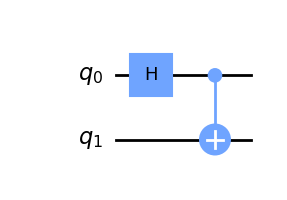
\includegraphics[scale=0.69]{./Bell_states_creation.png} 
\end{center} 
\caption{Circuito cuántico para la creación de estados de Bell}
\label{fig::NOT_gate}
\end{figure}\\
Esto equivale a 
\begin{equation}
\text{CNOT}\bigg((H_A\otimes\mathbb{1}_B)|ij\rangle_{AB} \bigg)
\end{equation}
con $i,j\in\{0,1\}$, para entender paso a paso este circuito o cálculo se presenta la siguiente tabla en donde se desglosa la evolución de estado inicial a través del circuito cuántico
\begin{center}
\begin{tabular}{ |c|c|c| } 
 \hline
 Estado Inicial $|ij\rangle_{AB} $ & $(H_A\otimes\mathbb{1}_B)|ij\rangle_{AB}$ & Estados de Bell \\ \hline
 $|00\rangle$  & $\frac{1}{\sqrt{2}}(|00\rangle+|10\rangle)$   &  $\frac{1}{\sqrt{2}}(|00\rangle+|11\rangle)$\\\hline
 $|01\rangle$  & $\frac{1}{\sqrt{2}}(|01\rangle+|11\rangle)$   &  $\frac{1}{\sqrt{2}}(|01\rangle+|10\rangle)$\\\hline
 $|10\rangle$  & $\frac{1}{\sqrt{2}}(|00\rangle-|10\rangle)$   &  $\frac{1}{\sqrt{2}}(|00\rangle-|11\rangle)$\\\hline
 $|11\rangle$  & $\frac{1}{\sqrt{2}}(|01\rangle-|11\rangle)$   &  $\frac{1}{\sqrt{2}}(|01\rangle-|10\rangle)$\\
 \hline
\end{tabular}
\end{center}
\subsection{Medición de Bell}
Como se ha mencionado varias veces se tiene que los circuitos cuánticos son reversibles, por lo que para ir en el sentido contrario al circuito de creación de Bell que se presentó anteriormente se introduce un circuito cuántico conocido como medición de Bell, que revierte el proceso, el circuito esta definido como 
\begin{figure}[h]
\begin{center}
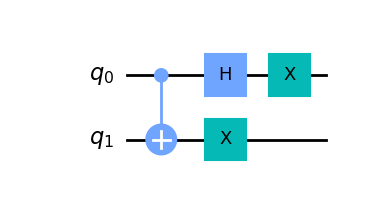
\includegraphics[scale=0.69]{./Bell_measurement.png} 
\end{center} 
\caption{Circuito cuántico para la medición de Bell}
\label{fig::Bell_measurement}
\end{figure}\\
Esto equivale a 
\begin{equation}
(\sigma_x\otimes\sigma_x)(H\otimes\mathbb{1})(CNOT|\psi^{ij}\rangle)
\end{equation}

\section{Teletransportación cuántica}
El objetivo del protocolo de teletransportación cuántica es el siguiente, Alice quiere enviar un estado cuántico $|\phi\rangle_S$(desconocido por Alice)
\begin{equation}
|\phi\rangle_S=\alpha|0\rangle_S+\beta|1\rangle_S
\end{equation}\\
a Bob, sin embargo solo puede enviar dos bit clásicos, aunque Alice supiera el estado es decir los valores reales de $\alpha$ y $\beta$, dos bits clásicos no son suficientes para codificar dos números reales. Sin embargo utilizando las propiedades cuánticas del entrelazamiento se puede lograr el objetivo de Alice.
Supongamos que Alice y Bob comparten un estado de Bell máximamente entrelazado 
\begin{equation}
|\psi^{00}\rangle_{AB}=\frac{1}{\sqrt{2}}(|00\rangle_{AB}+|11\rangle_{AB})
\end{equation}\\
Con esto se tiene que el estado inicial del sistema es 
\begin{equation}
|\phi\rangle_S\otimes |\psi^{00}\rangle_{AB}=\frac{1}{\sqrt{2}}(\alpha|000\rangle_{SAB}+\alpha|011\rangle_{SAB}+\beta|100\rangle_{SAB}+\beta|111\rangle_{SAB})
\end{equation}
Se nota que este estado inicial se puede reescribir como
\begin{equation}
\begin{split}
|\phi\rangle_S\otimes |\psi^{00}\rangle_{AB}=\frac{1}{\sqrt{2}}\bigg[ (|00\rangle_{SA}+|11\rangle_{SA})\otimes(\alpha|0\rangle_B+\beta|1\rangle_B)+(|01\rangle_{SA}+|10\rangle_{SA})\otimes(\alpha|1\rangle_B+\beta|0\rangle_B) \\
+(|00\rangle_{SA}-|11\rangle_{SA})\otimes(\alpha|0\rangle_B-\beta|1\rangle_B)+(|01\rangle_{SA}-|10\rangle_{SA})\otimes(\alpha|1\rangle_B-\beta|0\rangle_B)\bigg]
\end{split}
\end{equation}
Y esto equivale utilizando las definiciones de los estados de Bell(\ref{eq::bell1}, \ref{eq::bell2}, \ref{eq::bell3}, \ref{eq::bell4}) a 
\begin{equation}
|\phi\rangle_S\otimes |\psi^{00}\rangle_{\small{AB}}=\frac{1}{\sqrt{2}}\bigg[|\psi^{00}\rangle_{SA}\otimes|\phi\rangle_B+|\psi^{01}\rangle_{SA}\otimes\sigma_x|\phi\rangle_B +|\psi^{10}\rangle_{SA}\otimes\sigma_z|\phi\rangle_B+|\psi^{11}\rangle_{SA}\otimes\sigma_x\sigma_z|\phi\rangle_B \bigg]
\end{equation}\\

Con estos resultados es posible establecer un protocolo de teletransportación cuántica como se ve en la figura \ref{fig::qt_protocol}.
\begin{figure}[h]
\begin{center}
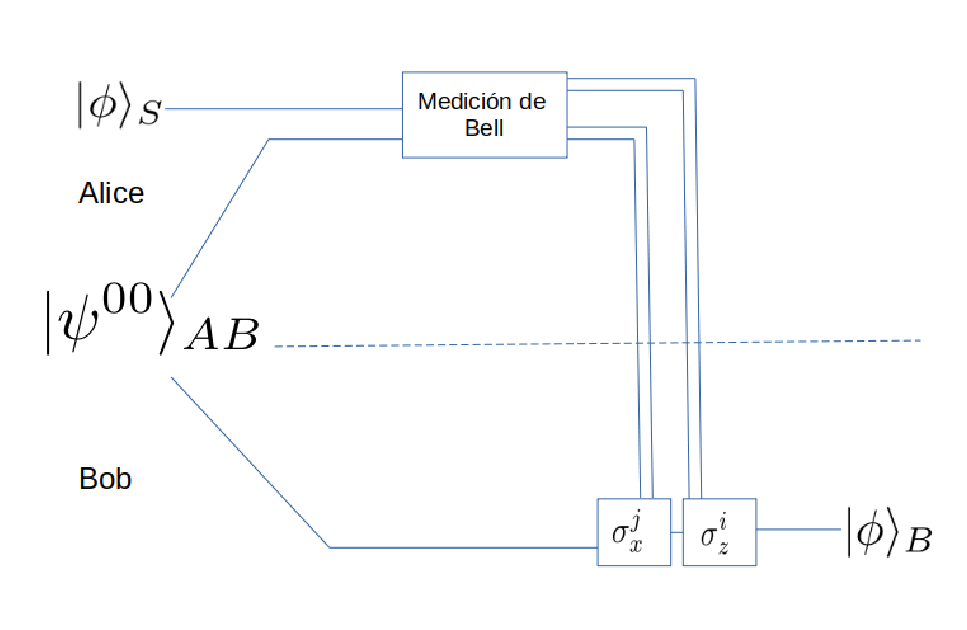
\includegraphics[scale=0.20]{./teletransportation_protocol.png} 
\end{center} 
\caption{Protocolo de teletransportación cuántica.}
\label{fig::qt_protocol}
\end{figure}\\
\linebreak
\pagebreak
\newpage
Los pasos del protocolo son los siguientes:
\begin{enumerate}
\item Alice mide al sistema SA en la base de Bell, para ver como funciona esto se presenta la siguiente tabla
\begin{center}
\begin{tabular}{ |c|c| } 
 \hline
 Alice Mide & Estado de Bob\\ \hline
 $|\psi^{00}\rangle$  & $|\phi\rangle_B$\\\hline
 $|\psi^{01}\rangle$  & $\sigma_x|\phi\rangle_B$\\\hline
 $|\psi^{10}\rangle$  & $\sigma_z|\phi\rangle_B$\\\hline
 $|\psi^{11}\rangle$  & $\sigma_x\sigma_z|\phi\rangle_B$\\
 \hline
\end{tabular}
\end{center}

\item Alice envía el resultado de la medición de Bell a Bob, es decir le envía dos bits clasicos $i,j \in \{0,1\}$.
\item Bob aplica $\sigma_z^i\sigma_x^j$ a su estado y obtiene $|\phi\rangle_B$
\end{enumerate}
Hay que notar que cuando Alice hizo la medición de Bell su estado colapsó, por lo que ya no  tiene al estado inicial $|\phi\rangle$, esto es de esperarse debido al teorema de no-clonacion de la mecánica cuántica, no puede copiar su estado, solo puede enviarlo a Bob destruyendo su estado en el proceso.

%En este trabajo de graduación consta de dos partes, en la primera parte se ha realizado una investigación sobre el enfoque de la mecánica estadística en la redes neuronales. En la segunda parte
\begin{thebibliography}{99}
%% La bibliografía se ordena en orden alfabético respecto al apellido del 
%% autor o autor principal
%% cada entrada tiene su formatado dependiendo si es libro, artículo,
%% tesis, contenido en la web, etc

\bibitem{Bell} J.S. Bell. \textit{On the Einstein Podolski Rosen Paradox}. \url{https://cds.cern.ch/record/111654/files/vol1p195-200_001.pdf}

\bibitem{Nielsen} Michael A. Nielsen, Isaac L. Chuang. \textit{Quantum Computation adn Quantum Information}. Cambridge University Press 2010. 10th. Anniversary Edition.

\bibitem{Feynman} Richard P. Feynman. \textit{Simulating Physics with Computers.} \url{https://doi.org/10.1007/BF02650179}.

\bibitem{Qiskit} \textit{Qiskit Textbook}. \url{https://qiskit.org/textbook-beta}

\bibitem{Mermin} N. David Mermin \textit{Quantum Computer Science: An Introduction}. Cambridge University Press, 2007.

\bibitem{Sakurai} J.J. Sakurai \textit{Modern Quantum Mechanics}. The Benjamin/Cummings Publishing Company, 1985.

\bibitem{Dotsenko} Viktor Dotsenko. \textit{An Introduction to the Theory of Spin Glasses and Neural Networks}. World Scientific 1994.

\bibitem{Bahri} Yasaman Bahri, Jonathan Kadmon, Jeffrey Pennington, Sam S. Schoenholz, Jascha Sohl-Dickstein, Surya Ganguli. \textit{Statistical Mechanics of Deep Learning}. \url{https://www.annualreviews.org/doi/pdf/10.1146/annurev-conmatphys-031119-050745}


\end{thebibliography}
\end{document}

